\documentclass[oneside,12pt,openany]{book}
\usepackage[toc,page]{appendix}
\usepackage{amsmath,amsthm,amsfonts,indentfirst,graphicx,subcaption,textcomp,commath,mathtools,hyperref,pgfplots,epigraph,enumitem,pdfpages}

\hypersetup{
	colorlinks=true,
	linkcolor=blue,
	filecolor=blue,      
	urlcolor=blue,
	citecolor=blue,
	bookmarks=true,
}

\usepackage{scrextend}
\usepackage{afterpage}
\newcommand\blankpage{
	\vfill
	\pagebreak
	\ifthispageodd{\null
		\vfill
		\vfill
		\clearpage}{}
}

\renewcommand{\baselinestretch}{1.5}
\setlength{\textwidth}{6in}

\newtheorem{defn}{Definition}
\newtheorem{thm}{Theorem}
\newtheorem{lemma}{Lemma}
\newtheorem{cor}{Corollary}
\newtheorem{prop}{Proposition}
\newtheorem{exa}{Example}
\newtheorem{clm}{Claim}
\newtheorem{rmk}{Remark}
\newtheorem{case}{Case}
\usepackage{mathtools}
\DeclarePairedDelimiter\ceil{\lceil}{\rceil}
\DeclarePairedDelimiter\floor{\lfloor}{\rfloor}

\begin{document}
	\begin{titlepage}
		\centering
		{\scshape\LARGE \textbf{An Exploration of the Topological and Logical Properties of Hierarchical Temporal Memory Networks} \par}
		{\scshape\LARGE Honors Research Proposal \par}
		\vspace{1cm}
		{\scshape\Large Alexander Michels\par}
		\vspace{0.5cm}
		{\scshape\Large Mathematics and Financial Economics\par}
		\vspace{0.5cm}
		{\scshape\Large Computer Science\par}
		\vspace{1cm}
		\vfill \large
		supervised by\par
		Dr.~Carolyn \textsc{Cuff}\par
		Dr.~C. David \textsc{Shaffer}\par
		Dr.~William \textsc{Procasky}\par
		
		\vfill
		
		% Bottom of the page
		{\large \today\par}
	\end{titlepage}
	
	\tableofcontents
	
	\newpage
	
	\chapter{Artificial Intelligence}
	
	\section{What is Intelligence?}
	
	Although we are continually bombarded with sensationalist news stories proclaiming the dawn and dangers of ``artificial intelligence,'' it is important to first define what it means to say a machine is intelligent. This is much the same way Turing began his preponderance of artificial intelligence in his 1950 \textit{Computing Machinery and Intelligence} \cite{Turing}. Turing came up with an eloquent boundary for determining the point at which we call a machine `intelligent.' His proposal, which he called ``The Imitation Game,'' but is now referred to as ``The Turing Test,'' is to have an interrogator question a human and an artificial intelligence, randomly labeled X and Y, in the hopes of distinguishing between the two \cite{Turing}. We reach ``intelligence'' when an interrogator cannot reliably distinguish between the two \cite{Turing}.
	
	As mathematicians, we could also take our favorite route of defining something: we look at a collection of things that we would agree to be ``intelligent'' and abstract the shared properties we consider to be desirable until we have a set of properties that must be met for a system to be considered intelligent. From this approach, we could say that a system \textbf{S} is intelligent if and only if it is able to ``use language, form abstractions and concepts, solves kinds of problems now reserved for humans, and improve themselves'' \cite{Jones}. This is the definition from the Dartmouth AI Summer Research Project, but such a definition is obviously hard to evaluate and it would be much more difficult to form a consensus on what set of properties define intelligence than it is to get a set of properties to define other abstract mathematical concepts such as an integral domain.
	
	It quickly becomes apparent that we also need more states than just the two Boolean ``intelligent''/``not intelligent'' ones to talk about intelligence in a constructive manner. Without this everything on the spectrum from a for loop with an if-else to the robots in Isaac Asimov's \textit{I, Robot}  are under the same label of ``not intelligent'' yet we know that the `intelligence' exhibited in those cases are not at all comparable. We need a spectrum with many states of intelligence to constructively talk about the intelligence of a system.
	
	John Searle's 1980 paper ``Minds, Brains, and Programs'' introduced the world to The Chinese room argument \cite{Searle}. It supposes that artificial intelligence research is successful and produces an artificial intelligence that is capable of behaving as if it understands Chinese, then asks does the machine literally understand Chinese or it simulating the ability to understand Chinese \cite{Searle}? Although this may seem like a pedantic distinction at first glance, the difference is truly important. The hypothesis that we can only ever simulate the ability to think is known as the weak AI hypothesis whereas the hypothesis that we can produce a machine capable of thought is the strong AI hypothesis \cite{Jones}. These both stand in contrast to Artificial General Intelligence, which is an intelligence capable of performing any intellectual task that a human can \cite{Buchanan}.
	
	\section{The History of Artificial Intelligence}
	
	
	One would think that artificial intelligence would have its roots in the last century or two, but mankind has dreamed of and proposed machines with human-like intelligence for thousands years, dating back to at least Homer \cite{Buchanan}. From our imagination and literature, artificial intelligence was brought into the realm of the academic by philosophers and mathematicians such as Ren\'e Descartes' ``mechanical man'' and Gottfried Wilhelm Leibniz's mechanical reasoning devices \cite{Buchanan}. Pascal and Leibniz both designed calculating machines capable of automated arithmetic, but proposing a calculator is far from what we think of as artificial intelligence today \cite{Buchanan}.
	
	It was the rise of electronics from Turing, IBM, Bell Laboratories, and countless others in the mid-twentieth century started to change the question from a philosophical one to a practical one \cite{Buchanan}. Artificial intelligence is a testament to the kind of interdisciplinary problem solving encouraged by the liberal arts, with contributions coming from the fields such as engineering, biology, psychology, game theory, communication theory, logic, philosophy, and linguistics \cite{Buchanan}. Advancements in computational power, operating systems, and language design allowed computer scientists to demonstrate computational problem solving such as Arthur Samuel's 1952 groundbreaking checker-playing program written in assembly language and one of the first examples of evolutionary computation \cite{Buchanan}. 
	
	Newell, Shaw, and Simon's ``Logic Theorist'' program became the first artificial intelligence written for a computer in 1956 \cite{Gugerty}. Through the use of heuristic algorithms, Logic Theorist was able to prove theorems and solve complex problems astonishingly well \cite{Gugerty}. These early attempts at artificial intelligence were largely doing two things: searching and finding ways to represent and manipulate knowledge. Claude Shannon pointed this out in his 1950 ``Programming a Computer for Playing Chess'' in which he produced what is now called the Shannon number, $10^{120}$, which is a lower bound of the game tree complexity of Chess \cite{Jones}.
	
	Artificial intelligence became formally recognized as a field of study and got its name from the 1956 Dartmouth Artificial Intelligence Conference \cite{Buchanan}. Another product of the conference was a step forward in artificial intelligence's ability to represent and manipulate knowledge with John McCarthy's development of the first AI programming language, LISP \cite{Jones}. The strides towards strong AI came crashing down with the publication of the 1969 paper ``Perceptrons'' which showed that single layer perceptrons were not able to properly handle linearly inseparable problems, leading to a steep decline in neural network research and ``AI Winter'' \cite{Jones}.
	
	Research into artificial intelligence reemerged in the mid to late eighties, but this time with a more practical focus rather than searching for Searle's strong AI \cite{Jones}. Algorithms developed and used for artificial intelligence found their way into camera auto-focus, anti-lock brakes, search engines, and medical diagnoses \cite{Jones}. Another marked difference is the plethora of approaches such as agent systems and biologically inspired systems. Today research into artificial intelligence has largely remained in this practical realm, using neural networks, data mining, fuzzy logic and other tools to solve real-world problems while slowly marching towards an Artificial General Intelligence.
	
	\section{Approaches to Artificial Intelligence}
	
	Artificial intelligence, because of how broadly the word can be defined and how many fields contribute the its progress, can be hard to wrap one's head around. However, Connell and Livingston have proposed four categories for artificial intelligence approaches which are useful for understanding the state of artificial intelligence research and the varied potential paths to Artificial General Intelligence \cite{Connell}.
	
	Their first category is labeled ``Silver Bullets'' and describes approaches in which much of what is needed is already believed to be present, but we are missing a crucial piece that will supposedly resolve our problems and deliver us a system with intelligence \cite{Connell}. Examples include `Fancy Logic' (second-order, non-monotonic, epistemic, deontic, modal, etc), Fuzzy Logic, Deep Language, Embodiment, and Quantum Computing \cite{Connell}. Disciples of this school of thought are chasing their particular ``Silver Bullet,'' working to formalize and perfect what they believe to be the missing link.
	
	They next describe the ``Core Values'' section which puts emphasis on the central organizational scheme over other computational details, believing that this macro-level structure has greater influence than the exact algorithms used \cite{Connell}. Situatedness, Emotionality, Self-Awareness, and Hierarchy \& Recursion are a few of these ideologies. There are strong arguments for this category, especially Hierarchy \& Recursions argument that an intelligence needs to be able to abstract recursively \cite{Connell}.
	
	Connell and Livingston's third category, ``Emergence,'' looks at artificial intelligence approaches which believe they already have the essentials, but we haven't implemented the essentials on a large enough scale to get our intelligence yet \cite{Connell}. For example, one might hold the position that intelligence is simply the ability to generate and search decision trees and we haven't realized an Artificial General Intelligence yet because our hardware doesn't allow us to do this effectively enough yet. Approaches in this category include Axiomatization, Commonsense, Learning, Evolution, and Integration \cite{Connell}.
	
	Lastly, we visit ``Emulation'' which is the school of thought that says we are better off copying intelligence than designing our own \cite{Connell}. Neural simulation, neural networks, animal models, human development, sociality, and cortical learning algorithms all fit in this category \cite{Connell}. The danger with this approach is abandoning theory in its sprint towards a functional copy, because if one does not understand the thing they have made, it is hard to see what it can do and where it can be improved. Another excellent point is that it can be very hard to correctly identify what needs to be copied, as Connell and Livingston note, ``artificial feathers and flapping turn out not to be needed to create airplanes'' \cite{Connell}.
	
	\chapter{Sparse Distributed Representations}
	
	Consider the binary representation of the integer 16 versus that of the integer 15. The two numbers are quite similar: they are only 1 apart, so they are as close as two integers can be. Yet their binary representations are [100000] and [011111] respectively. They have no shared ``on'' bits so despite their similarity, their binary representations reflect none at all. In fact, despite being as close as two integers can be (a Euclidean distance of 1), their binary representations have a Hamming distance, the number places in which two codewords differ, of 5, the maximum Hamming distance of two codewords of length 5 \cite{Adams}. 
	
	This means that our encoding does not preserve semantic similarity or a concept of distance between elements which is highly undesirable for an code because if there is some kind of error in the code we could end up decoding something meaning the opposite of what we were trying to convey. As an example, consider $\mathbb{Z}$ from 0 to 31 which is mapped to $GF(2)^{6}$ by their binary representation. The mapping of 31 is [111111] but a single error in transmission can easily lead to [011111] which would be decoded as 15. So a code Hamming distance ($d_{H}$) of one away ($\frac{1}{5}$ of the total metric) lead to an element 16 integers away ($\frac{1}{2}$ of the total metric). We would obviously like to avoid this so that errors in the transmission of our codes are either (1) correctable or (2) lead to a decoding that is as close as possible to our original element.
	
	This is achievable by simply conveying more information in our code. In our binary representation any single error led to another valid codeword (a codeword which decoded to an element of the input/output set) which meant that no errors could be detected or corrected. By expanding our code length, we increase the number of codewords (multiplying by the cardinality of the code alphabet for each character added) meaning that fewer errors will result in other valid codewords and can possibly be detected or corrected. 
	
	A key strategy with Sparse Distributed Representations is to encode semantic similarity, such as with our idea of distance in our motivating example. This helps us achieve our second goal because even if we increase the error-tolerance of our code, there is still some probability of an uncorrectable error and we would like that error to result in a codeword as close to the original codeword as possible. To give you a real world example imagine I am sending instructions to a aircraft and I need to tell it to turn down 17\textdegree to start its descent. Obviously, 18\textdegree or 16\textdegree are both preferable to 90\textdegree.
	
	To achieve our goal, we employ sparse distributed representations or SDRs. Just as with traditional dense binary representations, we will represent sparse distributed representations as vectors over their code alphabet, in this case GF(2). We call them \textbf{sparse} distributed representations because these vectors typically only have a small proportion of the components as 1. We will use Numenta's notation of letting $w_{\overrightarrow{x}}$ denote the number of components in an SDR $\overrightarrow{x}$ that are 1, so $w_{\overrightarrow{x}} = \norm{x}_{1}$ \cite{Properties}.
	
	Given our definition of distance, we could say that two decodings of sparse distributed representations, $a$ and $b$, are equal if and only if the $d_{H}(a,b) = w_{a} = w_{b}$. This would mean that both vectors would have to have the same dimensionality, same number of on bits, and all on and off bits would have to match. This definition is good for ``equals,'' but suppose we have a single error in transmission or a single component of our distributed system fails, equality would thus fail. In order to be able preserve the ability to subsample and thus to preserve fault tolerance, we therefore need a less stringent definition for decoding SDRs. Numenta refers to this as the $overlap$, which is $$ overlap(\overrightarrow{a}, \overrightarrow{b}) \equiv \overrightarrow{a} \cdot \overrightarrow{b} \equiv \sum_{0}^{n-1} a_{i}b_{i}$$ Thus, we say two SDRs $\overrightarrow{a}$ and $\overrightarrow{b}$ decode to the same element of the input space if and only if $overlap(a,b) \geq \theta$ where $\theta \leq w_{a}$ and $\theta \leq w_{b}$ \cite{Properties} I will call the function that determines if two sparse distributed representations decode to the same element of the input space using $\theta$ and $overlap(\overrightarrow{a}, \overrightarrow{b})$, $match_{\theta}(\overrightarrow{a}, \overrightarrow{b})$ and it is a function from SDR$\times$SDR $\longrightarrow$\{true, false\}.
	
	Given a set of sparse distributed representations with the same dimension, $X =\{\overrightarrow{x_{1}}, \overrightarrow{x_{2}}, ...,\overrightarrow{x_{n}}\}$, we can union the vectors using the bitwise OR operation over the $i^{th}$ position of the vectors in the set to produce the $i^{th}$ position of $union(X)$ \cite{Properties}. For example, given [0100] and [0010] the union would be [0110]. We say an SDR $\overrightarrow{y}$ is an element of the union of a set of SDRs, $\overrightarrow{X}$, if and only if $match_{\theta}(\overrightarrow{X},\ \overrightarrow{y})$ \cite{Properties}.
	
	\chapter{Hierarchical Temporal Memory}
	
	Hierarchical Temporal Memory is a technology that takes all the concepts we have briefly surveyed and combines them into a machine learning technology firmly rooted in the ``Emulation'' Path to Artificial Intelligence. It aims to capture the structure and algorithms of the neocortex in the hopes of delivering machines the intelligent though that the neocortex is thought to gift us \cite{Whitepaper}. Hierachical Temporal Memory networks (HTMs) are by definition a type of neural network, but are special because they model cells that are stacked in columns, which are organized in layers, in nodes, and in a hierarchy, following the layout of cells in the neocortex \cite{Whitepaper}.
	
	Hierarchical Temporal Memory follows what is known as a cortical learning algorithm \cite{Principles}. The cortical learning algorithm can be broken down into a few top level steps: initialization and encoding, the Spatial Pooler, the Temporal Pooler, and decoding the information. Of course, in a system with more than one level of regions, there is a hierarchy of regions with children regions feeding into parent regions to interpret multiple time series together which further complicates the network \cite{Dillon}. Bringing all of these complex pieces together yields Hierarchical Temporal Memory, but it is important to start by looking at what makes everything work: the cells.
	
	\section{Cells}
	
	The cell in a Hierarchical Temporal Memory network is the most basic building block from which the structure is formed. To understand how the system works, it is vital to first comprehend the internal structures and functions of the HTM's cells. They are comprised of three main components: synapses, the proximal dendrite, and the distal dendrites \cite{Whitepaper}.
	
	\begin{figure}[h!]
		\centering
		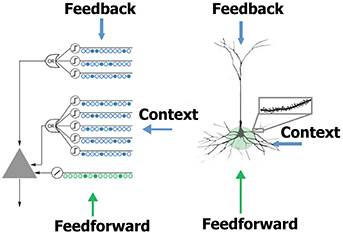
\includegraphics[width=\linewidth]{images/HTMCell.jpg}
		\caption{Hierarchical Temporal Memory Cell}
		\label{fig 1}
	\end{figure}
	
	Synapses in a Hierarchical Temporal Memory network represent a level of connection between two cells and are binary connected or not connected \cite{Whitepaper}. Although the connectedness of a synapse is binary, synapses have scalar ``permanence'' values which vary from 0.0 to 1.0 \cite{Principles}. A synapse is considered connected or valid when its permanence is above a certain threshold which is a parameter of the network, and permanence values are updated during the spatial pooling portion of the cortical learning algorithm \cite{Whitepaper}. Synapses are used by the proximal and distal dendrites.
	
	The proximal dendrite of a cell holds the synapses that bring a cell its feed-forward input \cite{Principles}. It only holds a set of potential synapses which represents a proper subset of all the inputs to the node and a cell's feed-forward activation is the sum of the activity of these synapses which will be discussed further \textbf{Spatial Pooler} \cite{Whitepaper}. Neurons that are arranged in the same column share a proximal dendrite so that they can receive the same feed-forward response which is a desirable property for reasons we will talk about later \cite{Whitepaper}.
	
	Cells also have a list of distal dendrite segments \cite{Whitepaper}. Each distal dendrite segment contains a list of potential synapses to other cells in the node. Segments learn by updating based on forming connections to cells that were active due to feed-forward input in the previous time step in order to predict its own cell's activation \cite{Whitepaper}. When a cell has a segment which has a number of active synapses above a threshold, the cell is considered to be in a predictive state \cite{Principles}.
	
	\section{Initialization and Encoding}
	
	Hierarchical Temporal Memory needs a way to move from the set of possible inputs, the input set, to the sparse distributed representations. This is accomplished by an encoding function which is specified from the input set to some $n$-dimensional sparse distributed representation. A region's input space and output space are the same; an HTM takes in a time series over the space and predicts an element or set of elements of the input space it believes to come next \cite{Purdy}. Each region has an input space which could be a single input set or the Cartesian product of multiple input sets. As an example, \{0,1,2,3,4\} could be an input set and if a parent region receives input from child region which has \{0,1\} as its input space and another child region with \{red, green, blue\} as its input space, then the parent region's input space would be \{(0, red), (1, red), (0, green), (1, green), (0, blue), (1, blue)\}. An encoding function from an input space to $n$-dimensional sparse distributed representations is not guaranteed to be surjective or injective. We would not expect surjectivity, but could get it through nearest neighbor decoding, but injectivity is something that one would think would be preserved. However, because parent regions are allowed to take a slice of the output vector (not the ``on'' bits, just an arbitrary portion) when being fed to from multiple child regions, we cannot guarantee the property.
	
	Before anything is sent through an HTM, each column is initialized with a list of initial potential synapses \cite{Whitepaper}. First we select a set of random inputs from the input set, then each input is represented by a synapse and given a random initial permanence value around the synapse validity threshold which are assigned such that each column has a bias towards the center of the input space \cite{Whitepaper}. Before we begin to send input to the system we also need an encoder which is a surjective function from the input space to our sparse distributed representations so that the HTM can interpret our time series.
	
	\section{Spatial Pooler}
	
	The Spatial Pooler is named so because the idea is to lump or pool together concepts that are semantically similar. It gives HTMs the ability to generalize and abstract. It accomplishes this through a couple of interesting steps that allow the system to preserve crucial information about the input in a sparse distributed representation but still generalize away some of the information in a algorithmic way. The fact that it is able to accomplish this through at all, let alone through the series of steps it takes is frankly incredible.
	
	The algorithm begins by computing the overlap that the input vector, $\overrightarrow{v}$, has with the particular column \cite{Whitepaper}. This can be accomplished by generating what I will call $\overrightarrow{pd}$, the vector of connected synapses on the proximal dendrite where ``1" represents a connected synapse and ``0" can represent either a potential synapse which is not in the subset held by the proximal dendrite but exists in the node's set of potential synapses or a potential synapse in the column's proximal dendrite's set of potential synapses which is not connected. The column's overlap field is initially set to $overlap(\overrightarrow{pd}, \ \overrightarrow{v})$. Then the columnn's overlap field is then compared to a minimum overlap parameter, and is set to zero if it is less than the parameter or multiplied by a boost function if the column's overlap field is greater than or equal to the parameter \cite{Whitepaper}.
	
	Next, the Spatial Pooler takes the set of columns with an overlap greater than zero and produces a subset that represents the most highly activated columns in each area of the node \cite{Principles}. This is accomplished with a desired local activity parameter which is used in conjunction with an inhibition radius to calculate a threshold at which its active overlap is high enough and if the overlap is greater than that threshold, it is added to the set of ``active'' columns \cite{Whitepaper}. The threshold is calculated by using the integer desired local activity parameter $desiredLocalActivity$, to find the overlap of the column with the $desiredLocalActivity^{th}$ highest overlap score \cite{Whitepaper}.
	
	Lastly, the algorithm performs its learning stage \cite{Whitepaper}. This consists of updating the permanence values of potential synapses in the proximal dendrite of each active column, updating the boost of each column, and updating the inhibition radius \cite{Whitepaper}. For each potential synapse in the proximal dendrite of each active column, the permanence is incremented by a parameter if the synapse is active and decremented by the parameter if not, but always bounded between [0,1] \cite{Whitepaper}. Then the algorithm calculates a minimum desired firing rate for each cell to adjust the cell's boost accordingly and the cell's synapse permanences can be increased by a scalar if the cell is not having large enough overlap using a sliding average \cite{Whitepaper}. The learning phase finishes by adjusting the inhibition radius in order to ensure that the representations the system will produce will be of the desired sparseness \cite{Whitepaper}.
	
	
	\section{Temporal Pooler}
	
	\begin{figure}[h!]
		\centering
		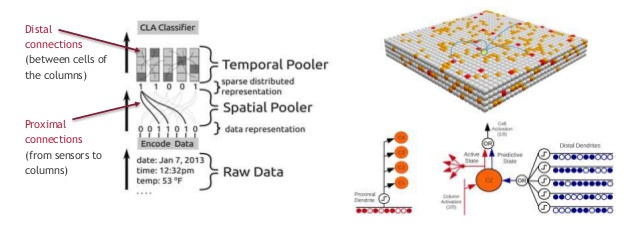
\includegraphics[width=\linewidth]{images/Poolers.jpg}
		\caption{Spatial and Temporal Poolers}
		\label{fig 2}
	\end{figure}
	
	The Temporal Pooler is named as such because its job is to pool together patterns through time series that it finds to be similar. Thus it is the Temporal Pooler's job to take the spatial patterns and attempt to find patterns through sequences of them \cite{Principles}. It is here that the cell structure of columns in HTMs matter because they allow the system to represent various patterns in different contexts \cite{Principles}. In an HTM node with 4 cells per column, 100 columns, and a 4\% activation rate, 4 columns represent each input, but each input can be represented $4^{4}=256$ ways. For example, the words ``eight" and ``ate" are homonyms and would be hard to tell apart if you heard the two without context, but in the sentences ``I ate a cookie" and ``I have eight pens" we are able to correctly distinguish between the two words solely because of their context.
	
	The first job of the Temporal Pooler is to decide which cell in the column should become active due to the column's activation \cite{Principles}. If any cells in the column were in a predictive state in the previous time step, we say those cells predicted the input, and those cells are chosen \cite{Whitepaper}. If none of the cells were in a predictive state, we put all of the cells in the column into a active state and the best matching cell for predicting the particular input is selected to be the learning cell and is given a new segment on its distal dendrite \cite{Whitepaper}. The idea behind making all the cells active is to say, ``We don't know how to interpret this, so all contexts are valid interpretations at this point'' \cite{Principles}.
	
	Secondly, the system needs to calculate the predictive state for each cell \cite{Whitepaper}. For each segment on the distal dendrite of each cell, if the segment is considered active, because enough of its synapses are active, the cell is put into a predictive state \cite{Principles}. The cell also has active synapses added to that that segment and another segment that has the best match to the activity in the previous time step in order to learn \cite{Whitepaper}. These changes are not immediately implemented however, they are queued up and when the next set of feed-forward input comes, if the cell is selected as a learning cell (its prediction was correct) it is positively reinforced, else if the cell stops predicting it is negatively reinforced \cite{Whitepaper}.
	
	\section{Hierarchy}
	
	The hierarchy of Hierarchical Temporal Memory comes from the ability to stack HTM regions in a tree like structure so that outputs of multiple HTM regions can be fed into a single parent region. So instead of interpreting the set of cells in a predictive state (that regions interpretation of its input) directly, we pass that information to another region with its own independent initialization. The parent region can also possibly receive another region's output or another raw input to contextualize the data. This ingenious structure comes from Jeff Hawkin's 2004 book ``On Intelligence,'' where he proposed that larger objects are composed of smaller objects (sentences of words, words of letters, etc.) and this structure allows lower regions to identify and predict the individual components and then higher regions to connect these components into more complex ideas \cite{Evaluation}.
	
	\section{Decoding}
	
	Once the system completes its processing of a time step's input, the system outputs a sparse distributed representation which may have gone through multiple layers and it is important to be able to decode the system's prediction in order for the system to be useful. Hierarchical Temporal Memory currently uses something called an SDR Classifier to decode the predictions of an HTM \cite{Dillon}. At its essence, an SDR Classifier is a single layer, feed forward, neural network \cite{Dillon}.

	\begin{figure}[h!]
		\centering
		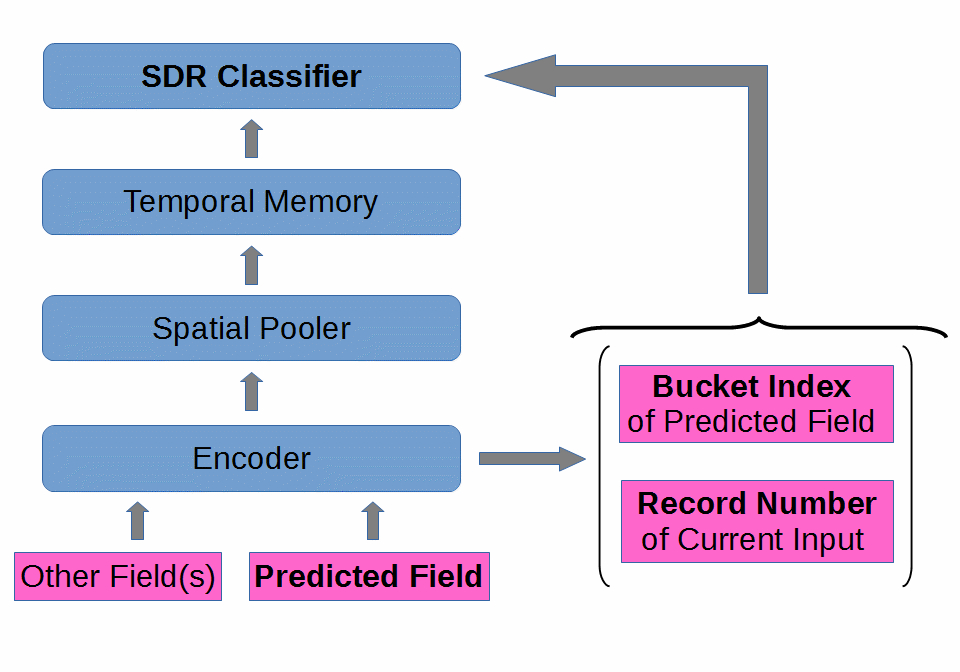
\includegraphics[width=\linewidth]{images/SDRClassifier.jpg}
		\caption{SDR Classifier}
		\label{fig 3}
	\end{figure}
	
	SDR Classifiers are able to decode the information HTMs give about predictions $n$ times steps in the future by maintaining a weight matrix \cite{Dillon}. The matrix's weights are adjusted to ``learn'' after each time step to reflect the correct weighting between the output vector at time $t$ and the probability distribution of the input/output space at time $t-n$ \cite{Dillon}. This enables the matrix to reflect relationships between inputs and outputs $n$ time steps apart. To determine the SDR Classifier's interpretation of an output at time $t+n$, the SDR Classifer takes in the HTM's output vector and uses Softmax to determine the most likely decoding \cite{Dillon}. So for each of the $k$ classes in the output space, the certainty that the output vector is referring to it is $$y_{j} = \dfrac{e^{a_{j}}}{\sum_{i=1}^{k} e^{a_{i}}}$$ where $a_{j}$ is the activation level of the $j^{th}$ element of the output space, calculated by multiplying the output vector by the $j^{th}$ column of the weight matrix element wise \cite{Dillon}. 
	
	
	
	\chapter{Literature Review}
	
	Hierarchical Temporal Memory has sparked a great amount of interest in the artificial intelligence community as everyone scrambles to ask how this biologically-inspired approach will fit into the Machine Learning landscape going forward. How do we mathematically formalize this emulation of the neocortex in order to integrate HTMs into the tools and systems we use today? How does their performance compare to the tools in use today when it comes to typical tasks like signal processing and forecasting? Will HTMs become an industry standard, fade to irrelevance, or somewhere in between? Much work has been done in this field and there is still much to be to done.
	
	Shortly after introducing the world to his theory of Hierarchical Temporal Memory, Jeff Hawkins along with Dileep George released a theory on the guiding mathematical principles in ``Towards a Mathematical Theory of Cortical Micro-circuits''. This mathematical framework is very high level, never diving past the node level of the HTM, but is quite interesting nonetheless. Under this model, Hierarchical Temporal Memory networks use Bayesian belief propagation as messages from one node represent a degree of certainly which is then used by the parent node to form its own inferences with their own degrees of certainty \cite{Towards}. They claim each node ``contains a set of coincidence patterns and a set of Markov chains defined over the set of coincidence patterns" \cite{Towards}. The framework is unable to describe how to convert the belief messages to the messages that a node sends to its children and although it is incredibly interesting this loose description of the system seems quite lacking.
	
	Some work has been done in formalizing the operation of the Spatial Pooler \cite{Framework}. This work related the algorithms, operations, and data structures of the Spatial Pooler to already existing ones, finding similarities in order to advance the computational efficiency \cite{Framework}. This mathematical framework is helpful for initializing and optimizing HTMs, but does not go as far as describing what a Hierarchical Temporal Memory network does to produce its forecasts.
	
	One of the applications of Hierarchical Temporal Memory that has been explored in some depth is its use in algorithmic trading. Many genetic algorithms and other methodologies for developing automated traders are only good at finding optimal parameters for their training data, but suffer once exposed to new data, a problem referred to as over-fitting. The hope is that Hierarchical Temporal Memory's ability to abstract spatial and temporal patterns will allow for the production of automated traders that are more resilient to over-fitting. Preliminary work in this field seems promising \cite{Evaluation}.
	
	An empirical study of Hierarchical Temporal Memory looked at its performance for biometric keystroke analysis, network data analysis, and website visitor analysis and concluded, ``that the predictions made by HTM models are clearly comparable, if not better, than the ones of the state-of-the-art approaches'' \cite{Galetzka}. The study also reaffirmed the conclusion of those using it for algorithmic trading, that HTMs are not very prone to over-fitting because they learn to generalize with more data \cite{Evaluation} \cite{Galetzka}. This study also found that finding the optimal parameters for an HTM is a very computationally intensive process because of the dependence of the parameters on each other making the search exponential in parameters that need to be optimized \cite{Galetzka}.
	 
	\section{Proposed Work}
	
	Hierarchical Temporal Memory is a branch of artificial intelligence grounded in Emulation, but I would like to take their strides in the field and see if can be improved using the innate topologies and inexact logic. I would like to implement my own Hierarchical Temporal Memory network using topological concepts to attempt to improve on the existing routines and enable broader logical frameworks to explore the performance and capabilities of such a system. Another possible advantage of using the topological properties is that I may be able to integrate topological or positional logic in order to enhance the system. Fuzzy logic and soft computing are another route I would like to take in improving Hierarchical Temporal Memory. It is my hope that this work will improve on the performance and forecasting ability of Hierarchical Temporal Memory.
	
	I am going to work on the coding and decoding process to attempt to find a better process for interpreting the output of a Hierarchical Temporal Memory network. It is my hope that a formal framework for cortical learning algorithms using topological concepts will enable me to build an algorithm which is better able to specify the range of likely predictions. Graph algorithms such as breadth first search on an undirected graph representing the output space and coding theory tools are just a few among the dozens of techniques we could try by reducing the problem to a more concrete one.
	
	I would like to use the floating point numbers and other non-Boolean values that are currently mapped to concrete states such as ``active"/``not active" and ``predictive"/``not predictive" and allow HTMs to work with them in these fuzzy states where cells will have degrees of activity. It is my hope that allowing the degrees of set membership and uncertainty to more explicitly propagate through the network, we will be able to extract the network's probabilistic beliefs about the subsequent time steps. Additionally, I believe that using prediction based on degrees of belief rather than Boolean belief will result in greater stability in the system as the system will be able to more readily adjust to new information in every time step leading to fewer paradigmatic changes resulting from Boolean shifts in lower regions.
	
	The first step in my research would be using topological properties present in Hierarchical Temporal Memory networks to attempt to improve upon the current decoding scheme. It is my hope that using the topological structures present we will be able to produce a more efficient or accurate decoding mechanism than Sparse Distributed Representation Classifier which essentially tracks the correlation between outputs and events. Using metric spaces and graph algorithms, I believe it is possible to build a decoding mechanism that first ``decodes'' the output with certainty as a function of distance in the metric space and then multiplies a vectors of probabilities that the output is referencing each element of the input space by a weight matrix to produce the prediction at time $n$. This would mean that the uncertainty of decoding would be dealt with in the graph algorithms and the weights in the weight matrix would not have to bare as much of the burden.
	
	The next step in my research would be to produce a fuzzy Temporal Pooler. The Temporal Pooler would keep the mechanism that decides which cell in a column should become active, but rather than a Boolean ``predictive''/``non-predictive'' state, cells would be able to represent a degree of predictive activity. There would be many challenges to overcome to accomplish this, such as changes to the learning mechanisms in the Temporal Pooler, possible changes to how the segments work, and whether the output for the cell is the raw activity level of the cell or possibly another value (such as a normalization using Softmax of the cells predictive states). The end result of this is to hopefully produce an HTM that can itself produce probabilistic predictions rather than relying on a probabilistic interpretation of its output.
	
	After this is done, I would like to reconcile this fuzzy Temporal Pooler with the rest of the system. This would mean producing a decoder that is able to handle the output of a fuzzy Temporal Pooler and convey which which uncertainties are a result of the probabilistic forecast and which are a result of an inexact decoding. From there it would be important to alter the Spatial Pooler to take in non-Boolean vectors for the system to work in a hierarchy. This could be done by mapping the vector to a Boolean vector or by altering the Spatial Pooler to allow for fuzzy logic.
	
	The hopeful net result will be a Hierarchical Temporal Memory network that is more flexible, more stable, and more capable. Failing that, this exploration will explore the uses of the innate topological structures in Hierarchical Temporal Memory, help us define the boundaries of what Hierarchical Temporal Memory may and may not be able to achieve, and explore if and how the concepts of fuzzy logic, fuzzy control, and soft computing can improve upon Hierarchical Temporal Memory.
	
	\newpage
	\addcontentsline{toc}{chapter}{References}
	\begin{thebibliography}{99}
				
		\bibitem{Adams} Adams, C and Robert Franzosa. 2008. \textit{Introduction to Topology: Pure and Applied}. Pearson Prentice Hall, Upper Saddle River, NY.
				
		\bibitem{Properties} Ahmad, S. and Jeff Hawkins. 2015. Properties of Sparse Distributed Representations and their Application to Hierarchical Temporal Memory. arXiv:1503.07469. Retrieved from https://arxiv.org/abs/1503.07469v1
		
		\bibitem{Evaluation} \r{A}slin, Fredrik. 2010. \textit{Evaluation of Hierarchical Temporal Memory in algorithmic trading}. Institutionen f\"{o}r Datavetenskap.
		
		\bibitem{Box} George E. P Box, Gwilym M. Jenkins. \emph{Time Series Analysis: Forecasting and Control, Fifth} (5th ed). John Wiley \& Sons, Inc., Hoboken, N.J., 2016.
		
		\bibitem{Buchanan} Buchanan, Bruce G. A (Very) Brief History of Artificial Intelligence. American Association for Artificial Intelligence, Volume 26, 53-60.
		
		\bibitem{Connell} Connell, Jonathan and Kenneth Livingston. Four Paths to AI. Frontiers In Artificial Intelligence and Applications, Volume 171, 394-398.
		
		\bibitem{Dillon} Dillon, A. 2016. SDR Classifier. Retrieved April 9, 2018 from http://hopding.com/sdr-classifier\#title
		
		\bibitem{Soft} Fortuna, L., et. al. 2001. \textit{Soft Computing: new trends and applications}. Springer-Verlag London, London, GB.
		
		\bibitem{Galetzka} Galetzka, Michael. 2014. \emph{Intelligent Predictions: an Empirical Study of the Cortical Learning Algorithm.} Master's thesis. University of Applied Sciences Mannheim. Mannheim, Germany. 
		
		\bibitem{Towards} George D, Hawkins J. 2009. Towards a Mathematical Theory of Cortical Micro-circuits. PLoS Comput Biol 5(10): e1000532. doi:10.1371/journal.pcbi.1000532 
		
		\bibitem{Gugerty} Gugerty, Leo. Newell and Simon's Logic Theorist: Historical Background and Impact on Cognitive Modeling. Proceedings of the Human Factors and Ergonomics Society Annual Meeting. Vol 50, Issue 9, pp. 880-884.  doi:10.1177/154193120605000904
		
		\bibitem{Whitepaper} Hawkins, Jeff, et al. Hierarchical Temporal Memory including HTM Cortical Learning Algorithms. Numenta, Version 0.2.1, 2011. 
		
		\bibitem{Jones} Jones, M. Tim. \emph{Artificial Intelligence: A Systems Approach}. Infinity Science Press, LLC, Hingham, M.A., 2008.
		
		\bibitem{Framework} Mnatzaganian, James, Ernest Fokoue, and Dhireesha Kudithipudi. A Mathematical Formalization of Hierarchical Temporal Memory's Spatial Pooler. Frontiers in Robotics and AI, Volume 3, Article 81.
		
		\bibitem{Munkres} Munkres, J. 2000. \textit{Topology} (Second Edition). Prentice Hall, Upper Saddle River, NJ.
		
		\bibitem{Advanced}. Numenta. 2008. Advanced NuPIC Programming. 
		
		\bibitem{Principles} Numenta. Principles of Hierarchical Temporal Memory (HTM): Foundations of Machine Intelligence. Video. (28 October 2014). Retrieved February 10, 2018 from https://www.youtube.com/watch?v=6ufPpZDmPKA
		
		\bibitem{Bayesian} Pelikan, M. 2005. \textit{Hierarchical Bayesian Optimization Algorithm}. Springer-Verlag Berlin Heidelberg, Germany.
		
		\bibitem{Purdy} Purdy, Scott. 2016. Encoding Data for HTM Systems. Computing Research Repository. arXiv: 1602.05925. Retrieved from: http://arxiv.org/abs/1602.05925
		
		\bibitem{Importance} Sangalli, A. 1998. \textit{The Importance of Being Fuzzy: and Other Insights from the Border between Math and Computers}. Princeton University Press, Princeton, NJ.
		
		\bibitem{Searle} Searle, John (1980), Minds, Brains and Programs, Behavioral and Brain Sciences, 3 (3): 417–457, doi:10.1017/S0140525X00005756, retrieved March 24, 2018
		
		\bibitem{Turing} Turing, A. M. Computing Machinery and Intelligence. Mind, Volume LIX, Issue 236, 1 October 1950, Pages 433–460, https://doi.org/10.1093/mind/LIX.236.433
		
		
	\end{thebibliography}
	
\end{document}